%Toy Falsification example
\todo[inline]{skipping for now}
We can also formulate a falsification problem \cite{AbbasATVA11_LinFalsification}, \cite{AbbasF_HybridSA12}, \cite{Deshmukh15_IterativeApproaches} by minimizing robustness in order to find trajectories of a closed loop system that violate a specification. In particular, we solve the following problem:

\begin{subequations}
\label{eq:falsification}
\begin{align}
\text{min}&_{x_0 \in X_0 } \, \rob_{\Psi}(\sstraj) \nonumber \\
\text{s.t. } & x_{k+1} = f_k(x_0) \, \forall k=0,\dotsc,N-1 \\
&  x_{k} \in X \, \forall k=1,\dotsc,N
\end{align}
\end{subequations}

For evaluation, we solve the problem for the point-mass system of \eqref{eq:PointMass}, with a state feedback controller for fixed-point tracking to the state $[2.25\,2.25]'$, which lies in the middle of the Terminal set (Fig. \ref{fig:toy falisification}). The specification is $\Psi=\always_{[0,20]} \neg (x_k \in \text{Unsafe})$, where the set $\text{Unsafe}$ is as defined earlier. The set of possible initial state, $X_0$ is shown in Fig. \ref{fig:toy falisification}, as is the initial point (used for initialization in the optimizer) and resulting trajectory, which satisfies $\Psi$ with a robustness of $1.25$. As before, $N=20$ is the length of the resulting trajectory under consideration.

For evaluation, we compare A) SQP using smooth robustness, B) SQP using Robustness and C) Simulated Annealing \cite{SABOOK}. Initial states and trajectories from the 3 methods are shown in Fig.\ref{fig:toy falisification}. Here. methods A) and B) result in the same initial state $x_0=[-2.3418\, -2.3418]'$, while C) gives $x_0=[-2.3371\, -2.3354]'$. The robustness for trajectories from both SQP based methods is $-0.99998$, while via Simulated Annealing is $-0.9968$. Note, the trajectories via either method are very close, and pass near the center of the $\text{Unsafe}$ set (the origin), where the robustness reaches its minima of $-1$. Also worth noting, that for the trajectory via method A), $\srob_{\Psi}=-0.9932$, i.e. a relative approximation error of less than $1\%$.

\begin{figure}[t]
\centering
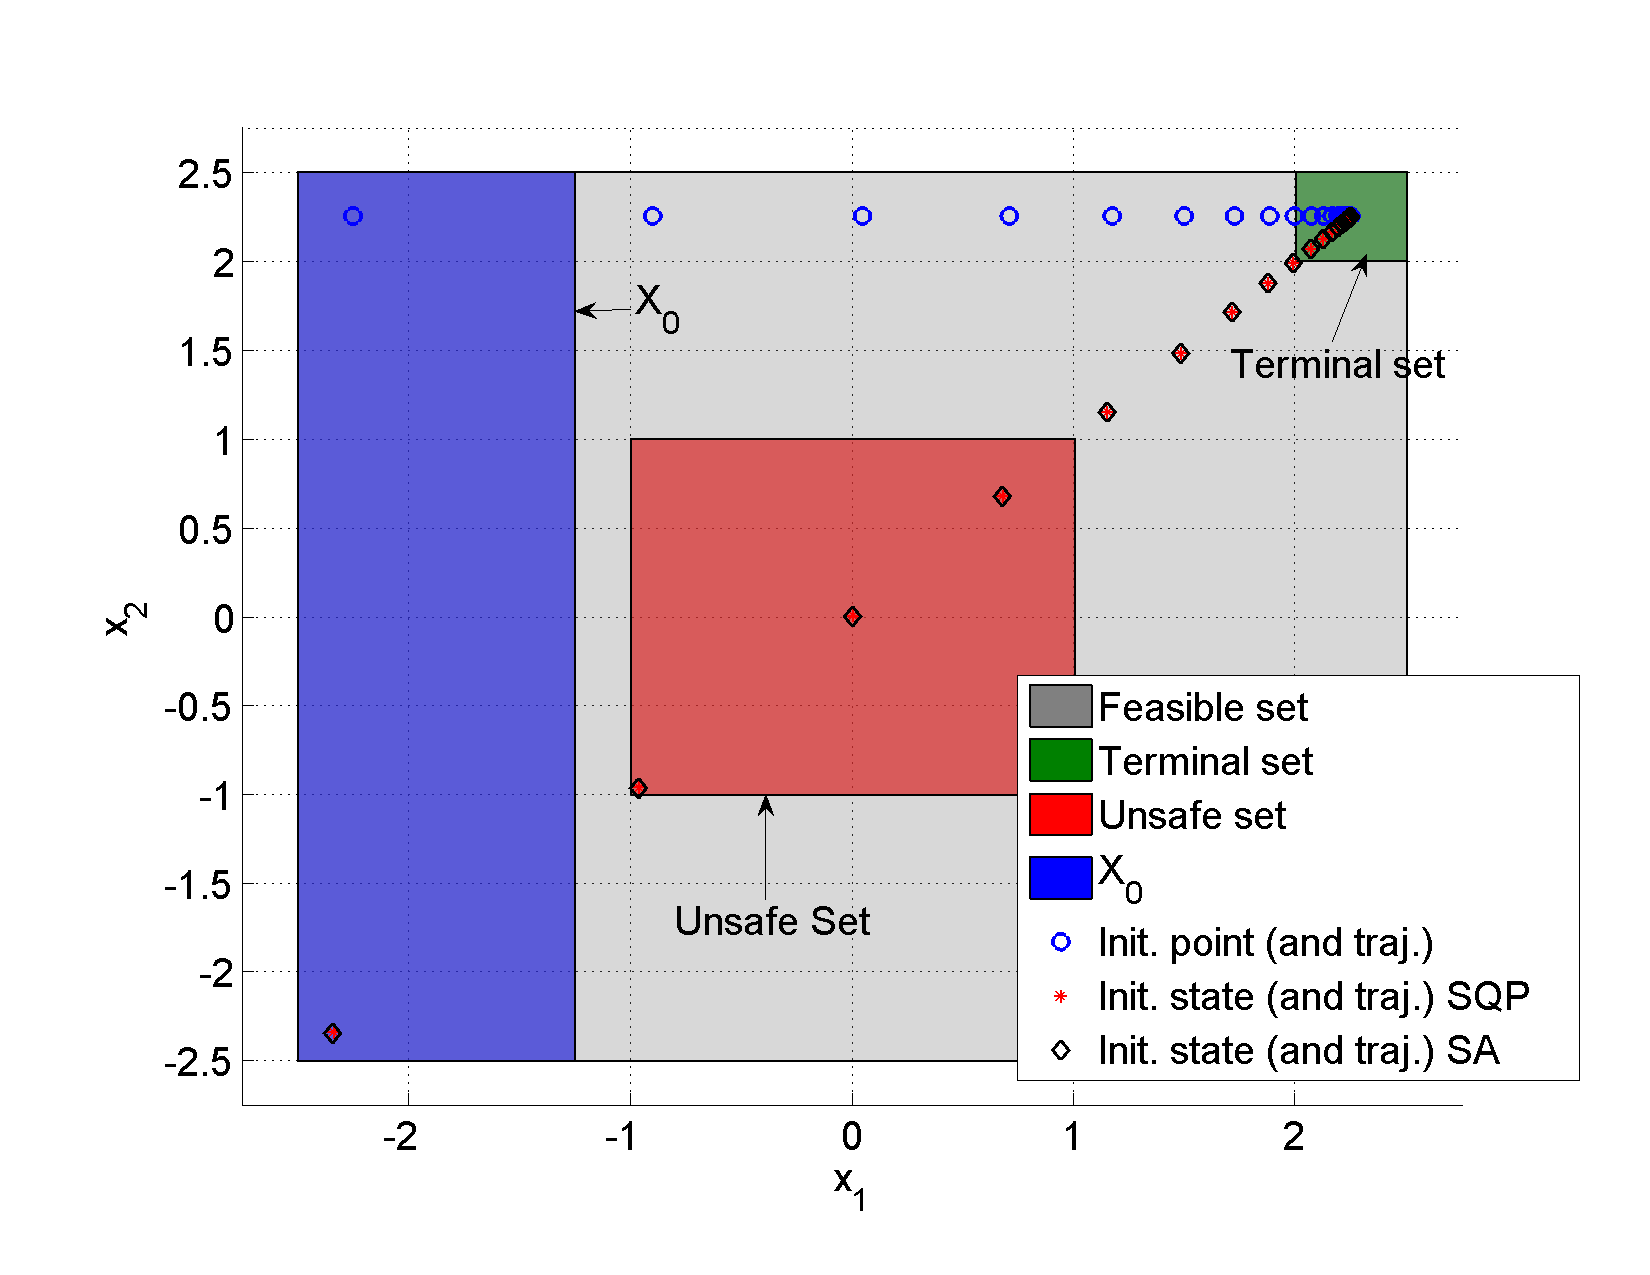
\includegraphics[width=0.49\textwidth]{figures/ToyExampleFalse}
\caption{Trajectories from initial points obtained from robustness minimization via Simulated Annealing (SA), SQP, and SQP on smooth robustness. Note, both SQP and SQP on smooth robustness lead to the same solution.}
\label{fig:toy falisification}
\end{figure}